\title[Systems Engineering]{ Systems Thinking  Part `1 } 



\newpage
\begin{frame}
\frametitle{ Systems Thinking  Part 2 }
\begin{block}{ Systems thinking originated :}


\colorbox{cyan}{ \textcolor{white}{1956 when Professor Jay Forrester  } }   founded the Systems Dynamic Group at MIT's Sloan School of Management.

\end{block}
\end{frame}


\newpage

\begin{frame}
\frametitle{ Systems Thinking  Part 2 }
\begin{block}{ Systems Thinker :}

 
\begin{figure}
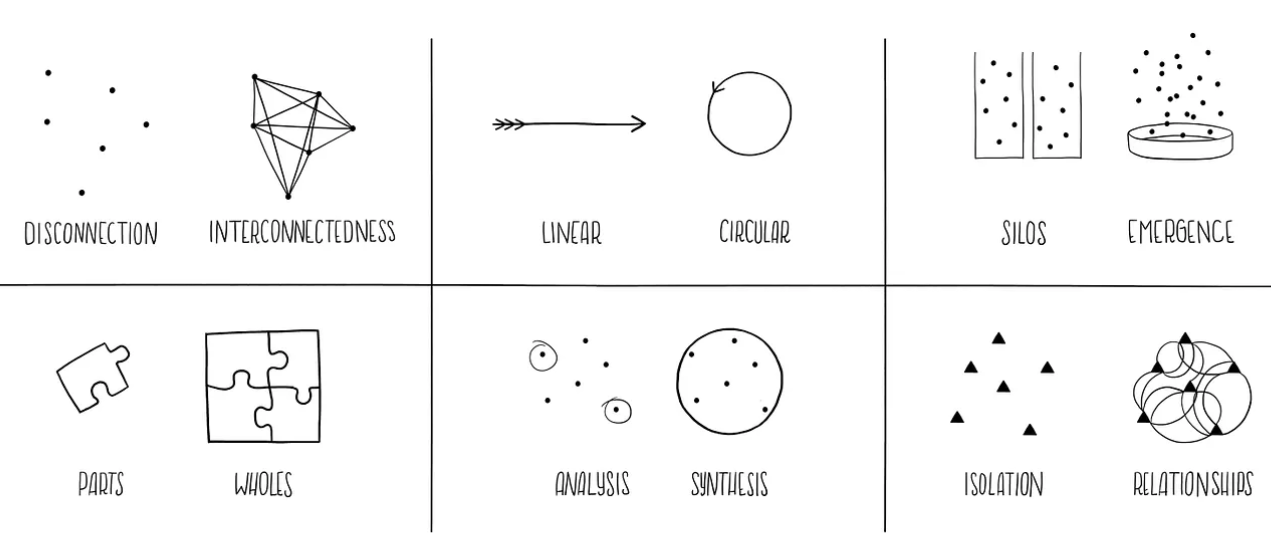
\includegraphics[scale=0.46]{pic/dthink1.png}
\caption{ Tool for Systems Thinker  }
\label{Layer1}
\end{figure}

\end{block}
\end{frame}





 
\newpage
\begin{frame}
\frametitle{ Systems Thinking  Part 2 }
\begin{block}{ Characteristics of systems thinking}

\vspace{0.5cm}

\framedtext{ 
\textcolor{teal}{
Systems thinking is a holistic approach to analysis that 
 focuses on the way that a system's constituent parts interrelate and how systems work over time and within the context of larger systems. }
}




\vspace{0.5cm}

\framedtext{ 
\textcolor{cyan}{
The systems thinking approach contrasts with traditional analysis, which studies systems by breaking them down into their separate elements.}
}

\end{block}
\end{frame}


\newpage

\begin{frame}
\frametitle{ Systems Thinking  Part 2 }
\begin{block}{ Micro vs Huge   }

 
\begin{figure}
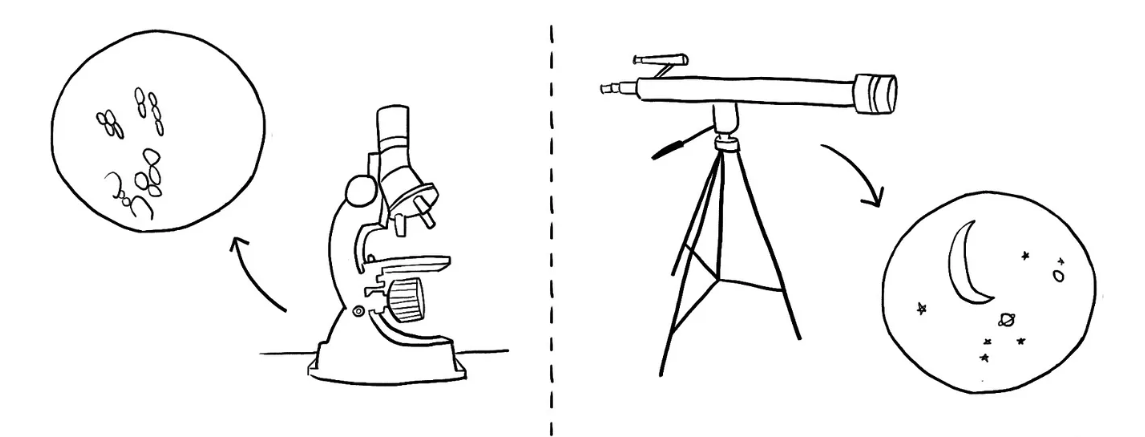
\includegraphics[scale=0.56]{pic/scale1.PNG}
\caption{ Scale for Systems Thinker  }
\label{Layer1}
\end{figure}

\end{block}
\end{frame}



\newpage
\begin{frame}
\frametitle{ Systems Thinking  Part 2 }
\begin{block}{ Assumptions and Questions}

\begin{enumerate}
    \item  Collect assumptions
    \item Set up the activity
    \item  \colorbox{red}{ \textcolor{white}{ Identify high-risk uncertainties } }  
    \item  Build an action plan
\end{enumerate}

\end{block}
\end{frame}


\newpage

\begin{frame}
\frametitle{ Systems Thinking  Part 2 }
\begin{block}{ Measure the GAP }

 
\begin{figure}
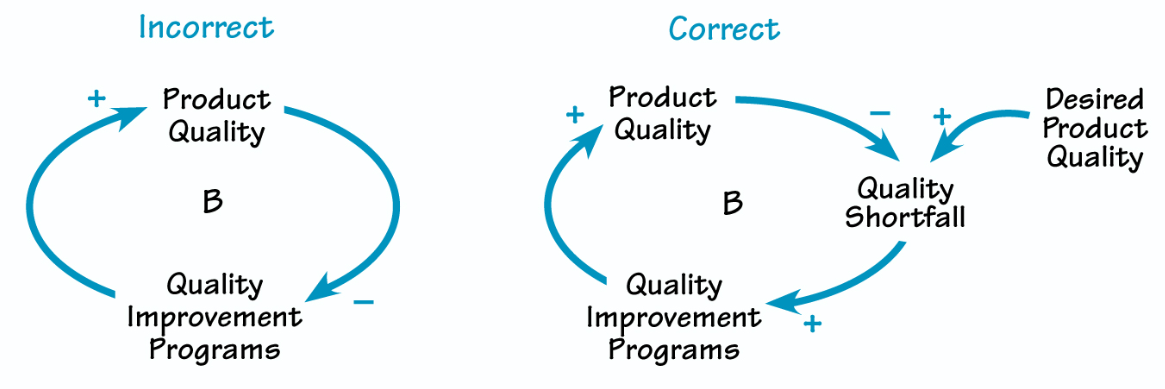
\includegraphics[scale=0.46]{pic/correct1.PNG}
\caption{  OLD and  Customer friendly NEW  }
\label{Layer1}
\end{figure}

\end{block}
\end{frame}


\newpage
\begin{frame}
\frametitle{ Systems Thinking  Part 2 }
\begin{block}{ Collect assumptions }


Diverge, with each team member writing one assumption or question per sticky note. Withhold judgement or discussion until later.

\url{https://www.overleaf.com/project/645a7be5a600eb8684ec131b}

\end{block}
\end{frame}



\newpage
\begin{frame}
\frametitle{ Systems Thinking  Part 2 }
\begin{block}{ Data and Sharing }

\begin{enumerate}
    \item  Set up the activity
    \item Start with the obvious
    \item  Find your data experts
    \item  Vote on the most critical data sources
\end{enumerate}

\url{https://www.ibm.com/design/thinking/page/toolkit/activity/ai-essentials-data}

\end{block}
\end{frame}



\newpage
\begin{frame}
\frametitle{ Systems Thinking  Part 2 }
\begin{block}{ Cognitive Walkthrough}

Observe users interacting with a prototype in order to evaluate its success.

\begin{enumerate}
    \item   Identify scenario and tasks
    \item  Prepare your prototype
    \item Test with users
    \item  Review and reflect
\end{enumerate}

\url{https://www.ibm.com/design/thinking/page/toolkit/activity/cognitive-walkthrough}

\end{block}
\end{frame}


\newpage
\begin{frame}
\frametitle{ Systems Thinking  Part 2 }
\begin{block}{ Framework}

Lead teams to great user outcomes using our scalable framework for team alignment.

\url{https://www.ibm.com/design/thinking/page/framework}

\end{block}
\end{frame}


\newpage
\begin{frame}
\frametitle{ Systems Thinking  Part 2 }
\begin{block}{ Reference}

 

\url{https://medium.com/disruptive-design/tools-for-systems-thinkers-the-6-fundamental-concepts-of-systems-thinking-379cdac3dc6a}

\url{https://thesystemsthinker.com/}

\end{block}
\end{frame}
